\begin{tikzfigure}
    \subcaptionbox{$\lambda = \lambda_{L} = 830$ nm.}{
        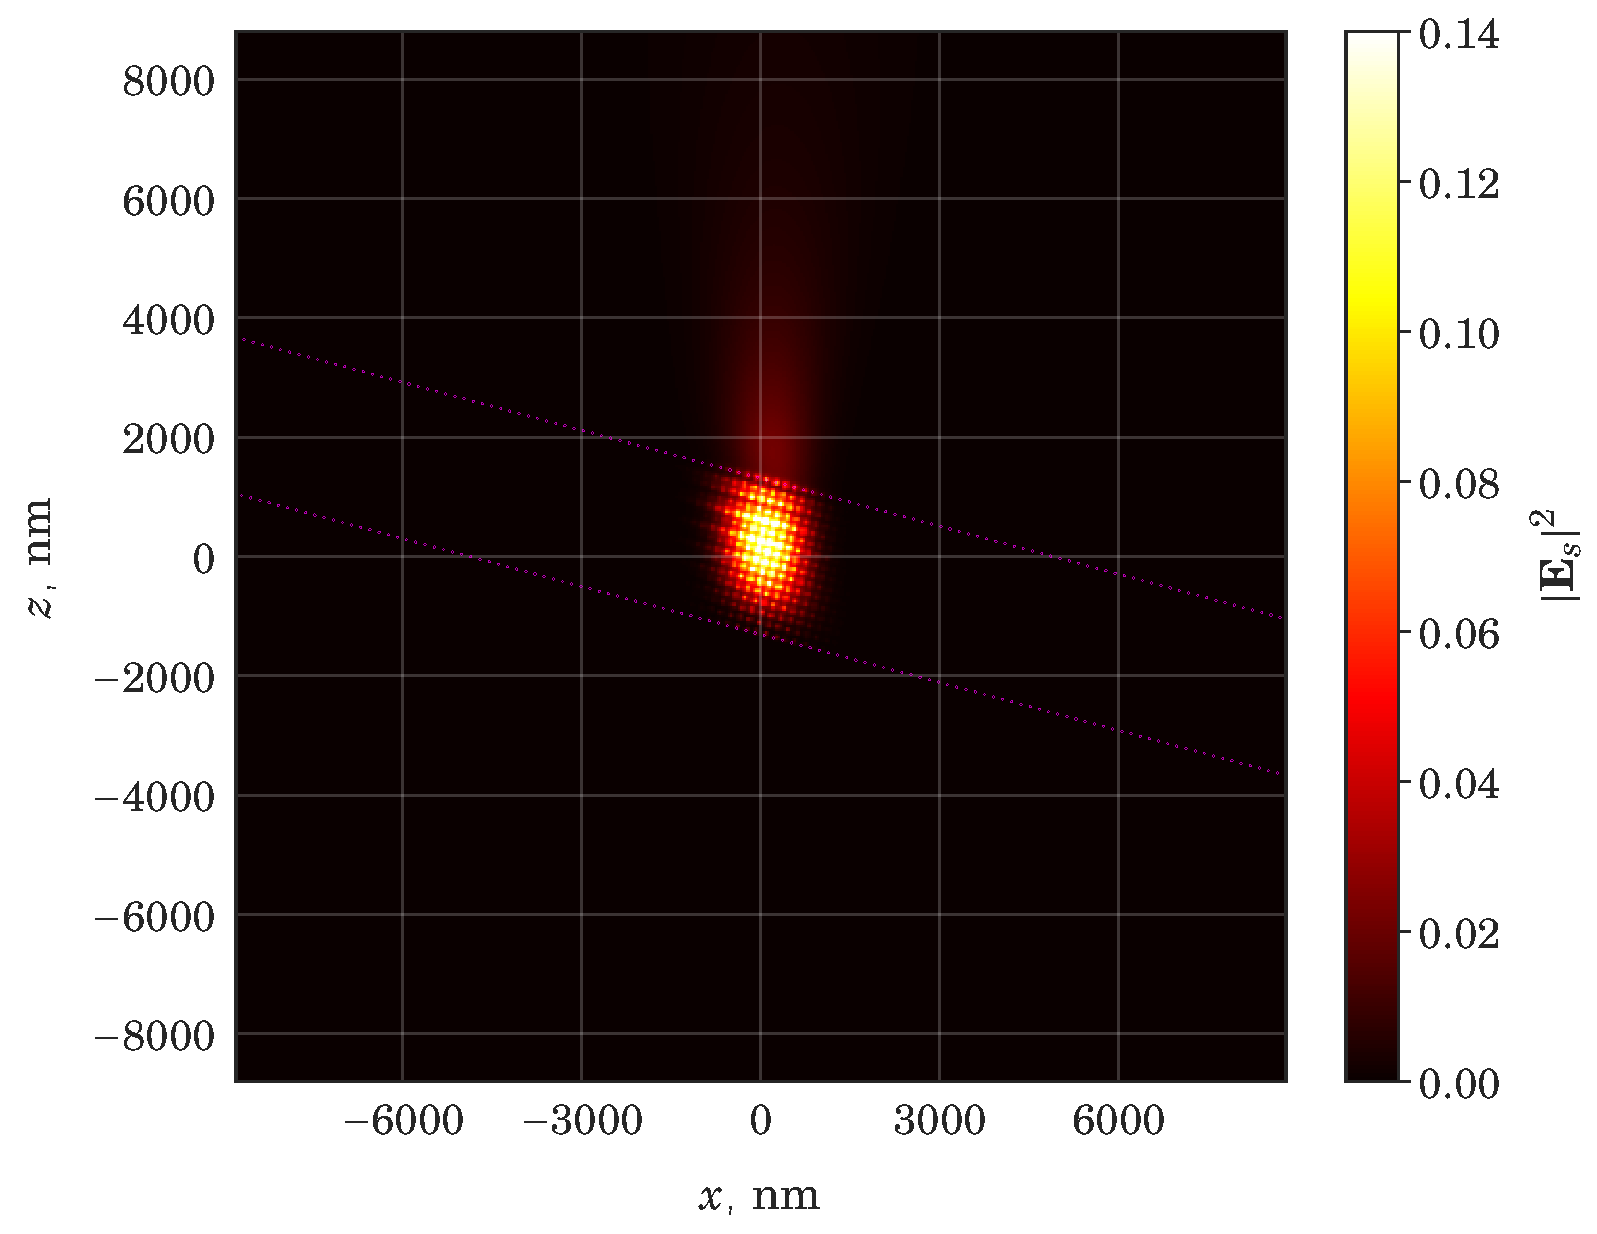
\includegraphics[width=0.45\linewidth]{../img/celes/Es_20nm_15deg_1harm.pdf}
    }
    \hfil
    \subcaptionbox{$\lambda = \lambda_{10} = 83$ nm.}{
        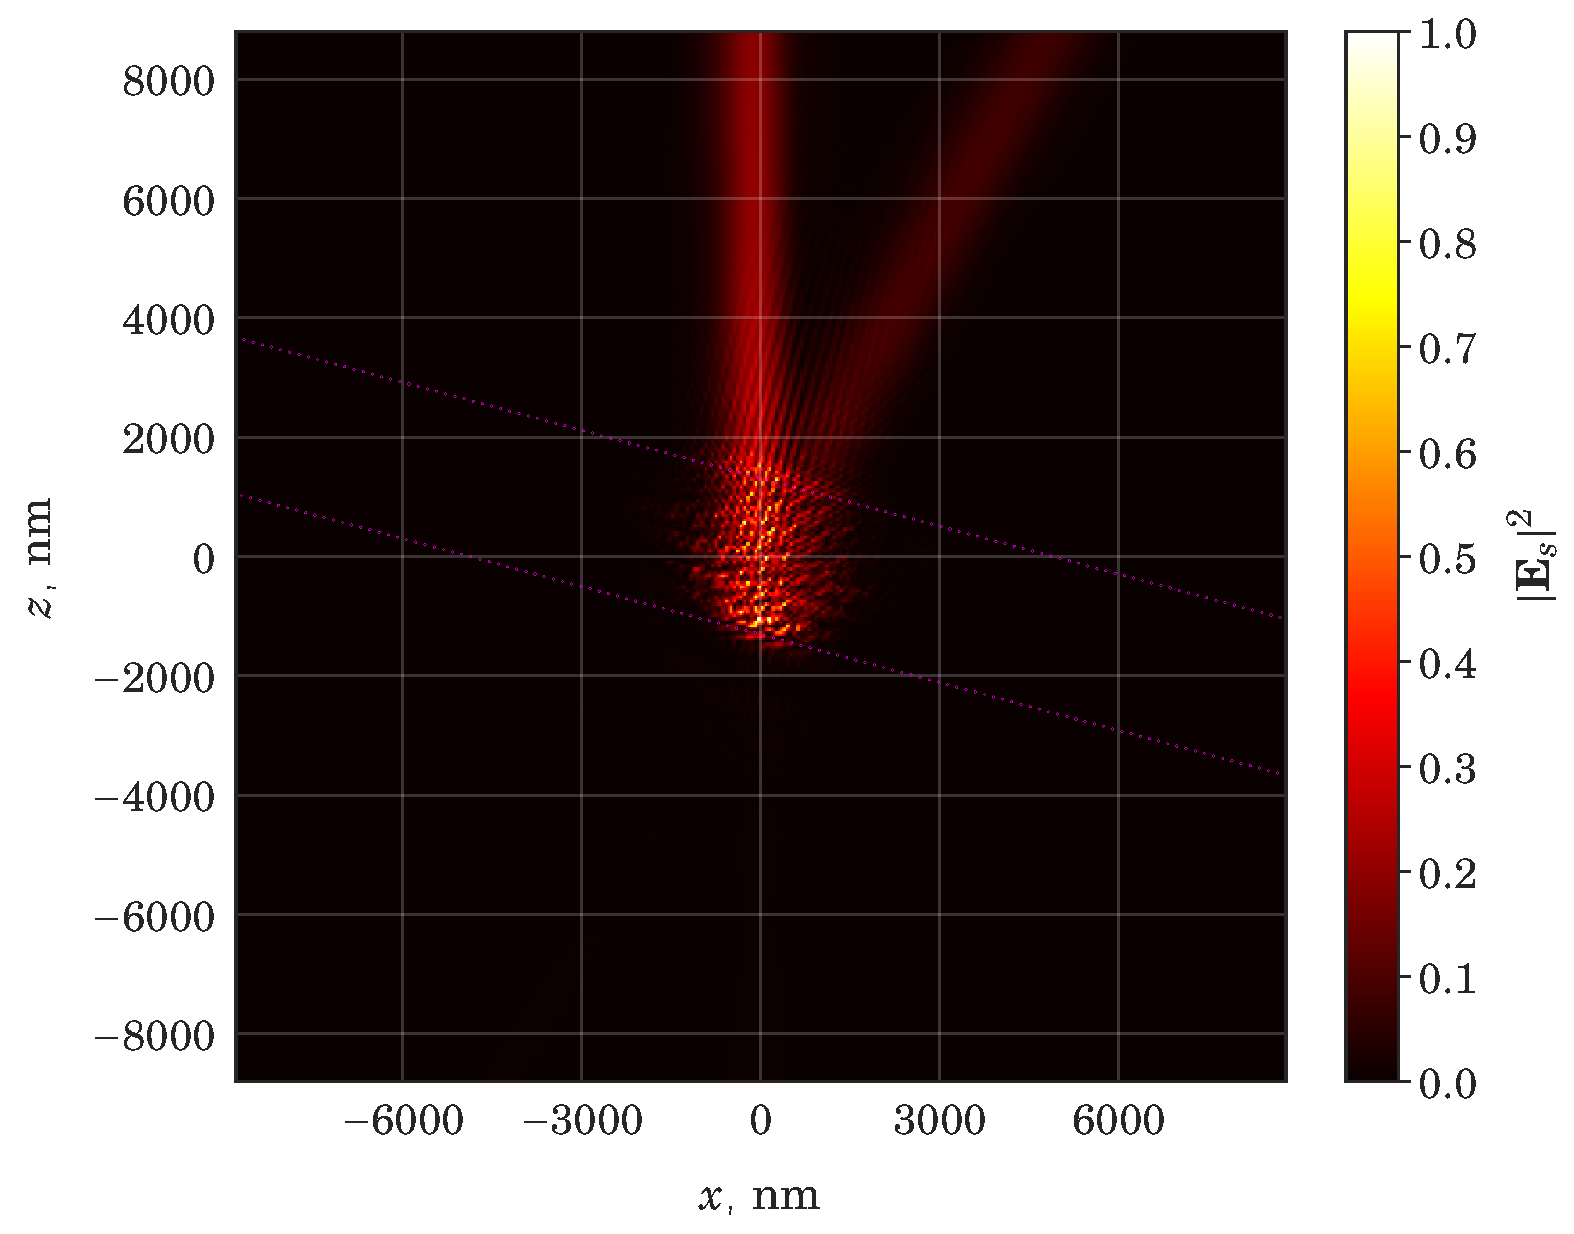
\includegraphics[width=0.45\linewidth]{../img/celes/Es_20nm_15deg_10harm.pdf}
    }
    \\
    \subcaptionbox{(\ref{bragg_wolf_order_spherical}) solution in integer Miller indices.}{
        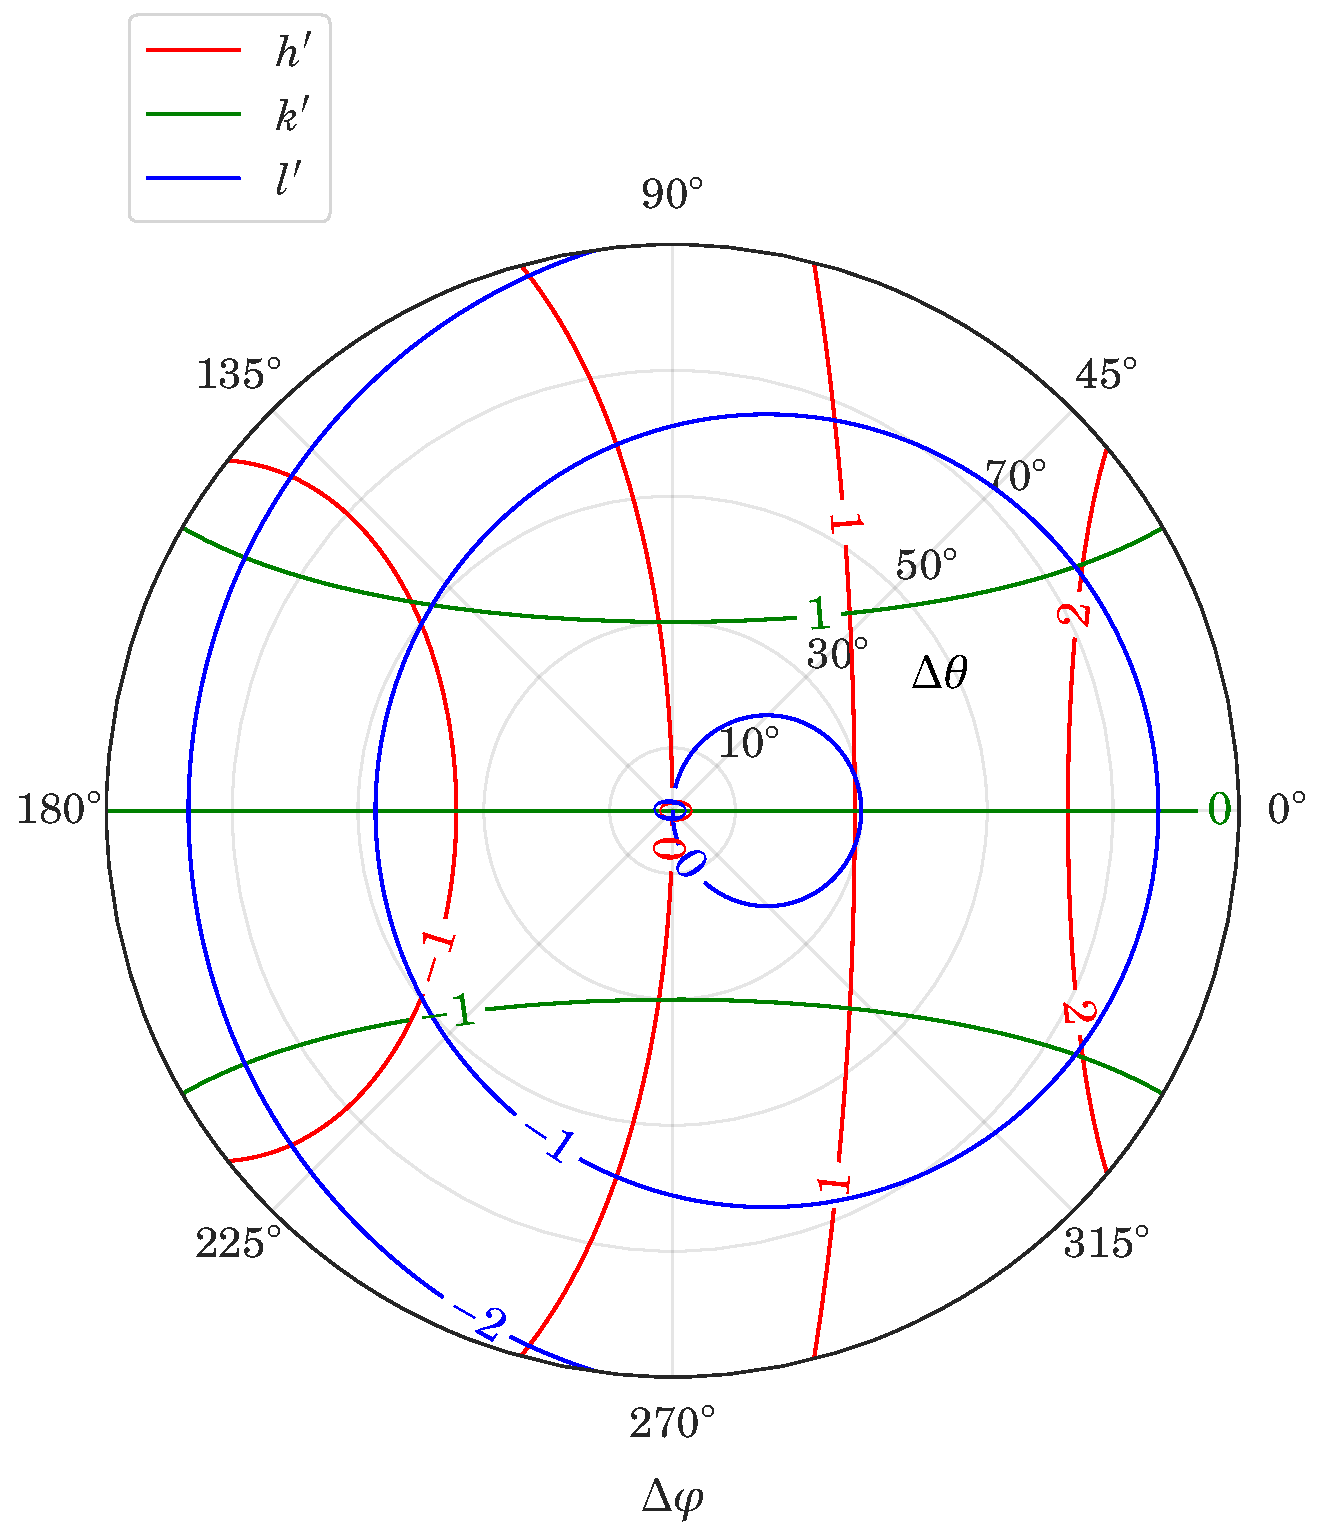
\includegraphics[width=0.38\linewidth]{../img/celes/dphi_dtheta_kprime_d_2l_phi0_0_theta0_15.pdf}
    }
    \hfil
    \subcaptionbox{$E_{\textrm{int}}$ from (\ref{e_int}).}{
        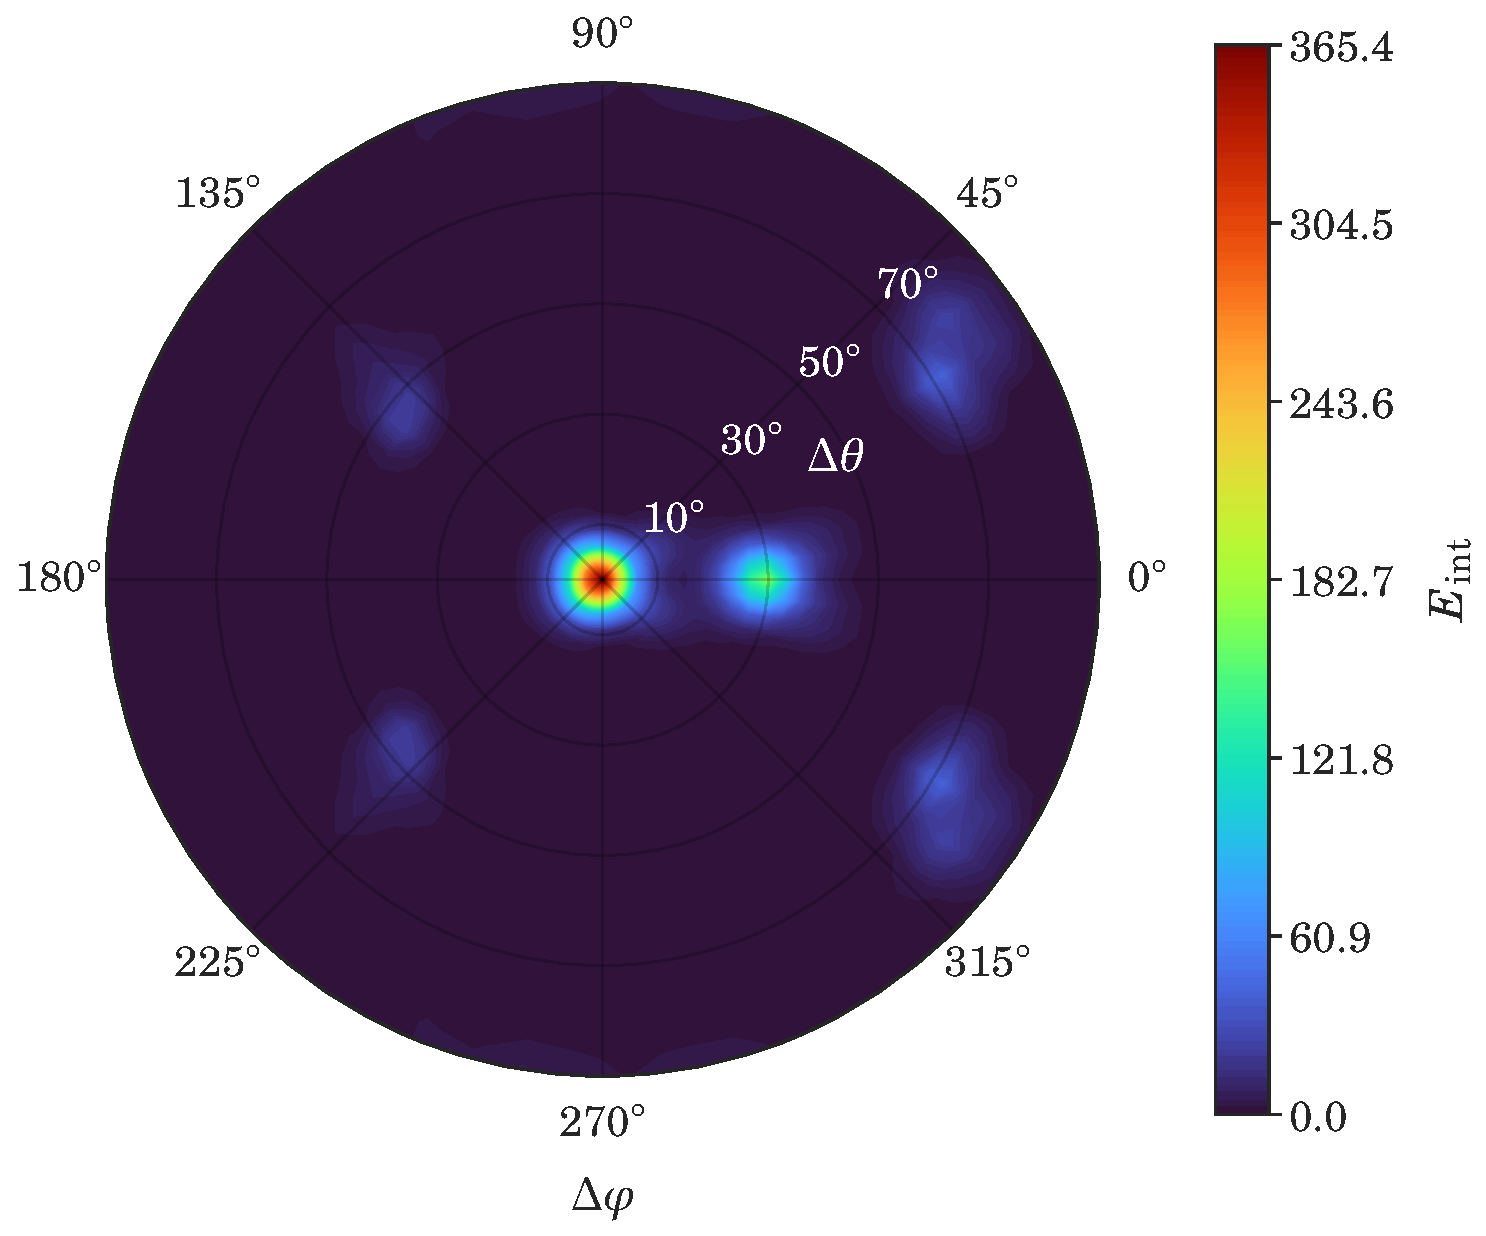
\includegraphics[width=0.48\linewidth]{../img/celes/E_squared/eint_10harm_15deg_0.0nonreg.pdf}
    }
    \label{1st_check_diffrth:image}\caption{10th harmonic scattering for $a = 20$ nm and $d = 2\lambda_{10}$, $\varphi_0 = 0^{\circ}$, $\theta_0 = 15^{\circ}$, $\lambda = \lambda_{10} = 83$ nm, $\Delta \theta \in \left[ 0,\:\pi\,/\,2 \right]$.}
\end{tikzfigure}

\begin{tikzfigure}
    \subcaptionbox{Impact of the target irregularity.}{
        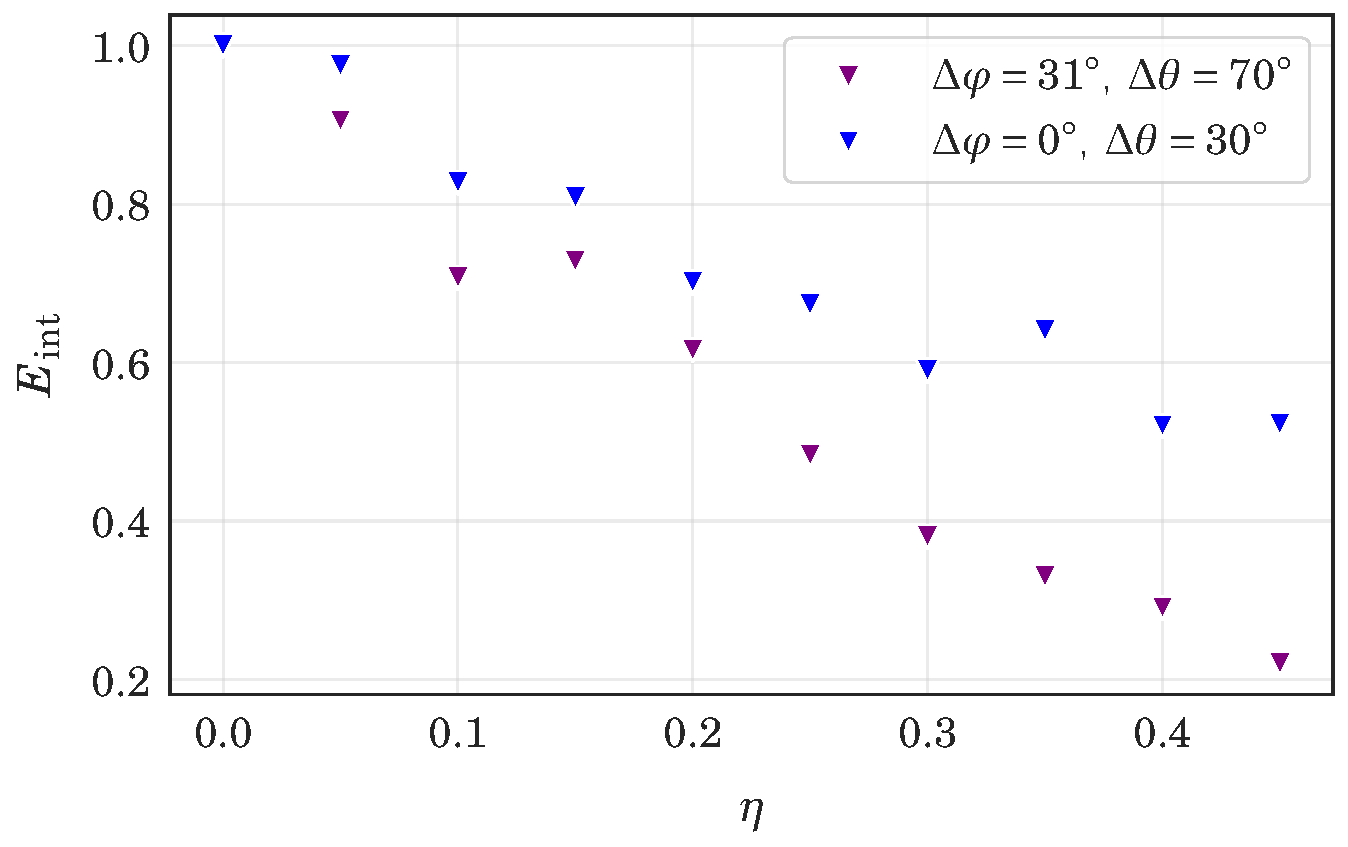
\includegraphics[width=0.48\linewidth]{../img/celes/energy_vs_nonreg}
    }
    \hfil
    \subcaptionbox{Impact of the cluster radius, values normalized to $E_{\textrm{int}}$ at $a = 20$ nm.}{
        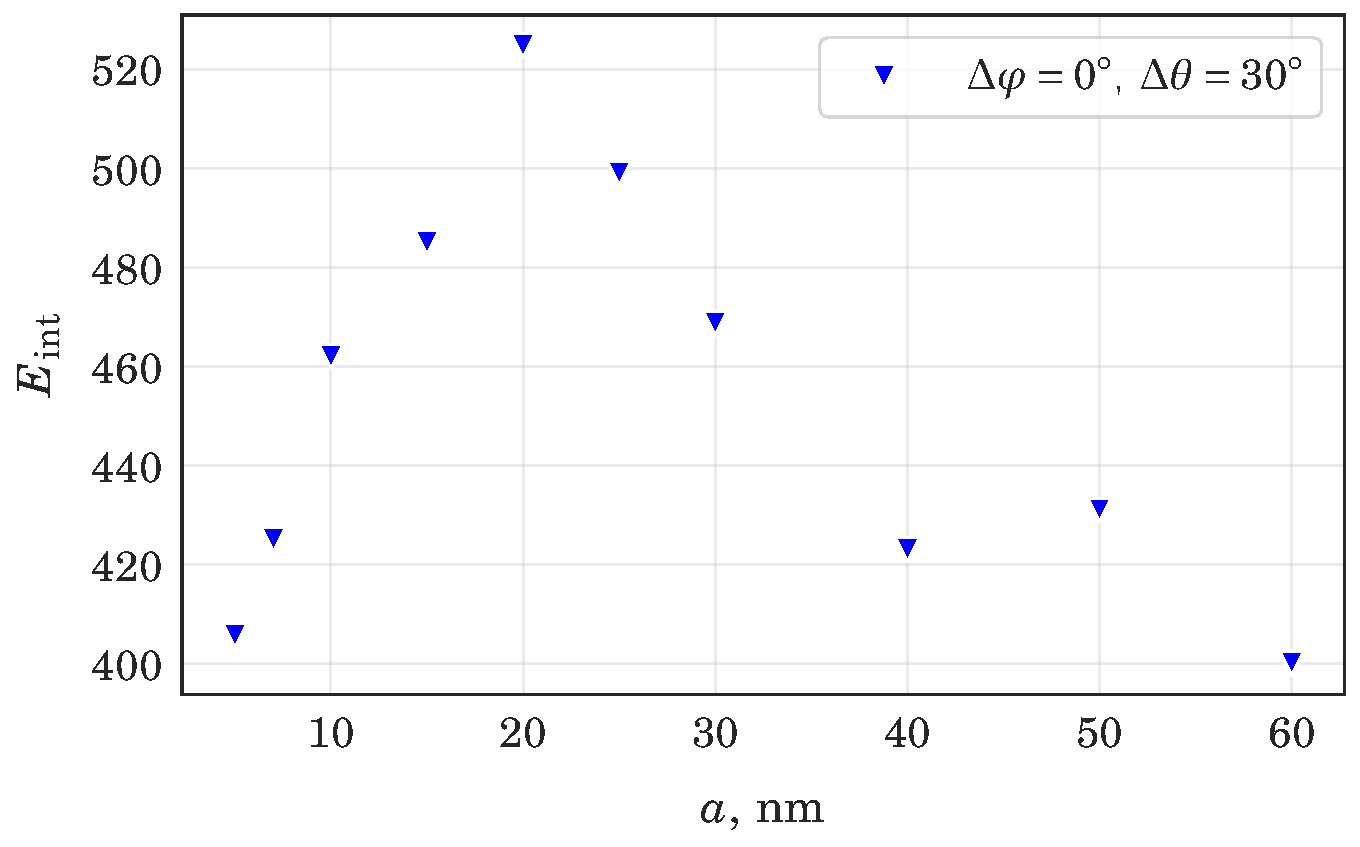
\includegraphics[width=0.48\linewidth]{../img/celes/energy_vs_radius}
    }
    \label{scat_at:image}\caption{Scattering attenuation depending on the target irregularity and the cluster radius.}
\end{tikzfigure}